%Įvade aprašomi darbo tikslai, nurodomas temos aktualumas, aptariamos teorinės
%darbo prielaidos bei metodologija, apibrėžiamas tiriamasis objektas,
%apibūdinami su tema susiję literatūros ar kitokie šaltiniai, temos analizės
%tvarka, darbo atlikimo aplinkybės, pateikiama žinių apie naudojamus
%instrumentus (programas ir kt.). Rekomenduojama įvado apimtis 3-4 puslapiai.

\sectionnonum{Įvadas}

% Kas yra biometrines identifikavimo sistemos
Kiekvieno žmogaus kūnas turi aibę savybių, kurios gali unikaliai jį identifikuoti (pvz.: pirštų atspaudai).
Šių savybių egzistavimas davė pagrindą {\it biometrinėms identifikavimo sistemoms}.
Biometrinio identifikavimo sistema yra tokia sistema, kuri geba palyginti kandidato biometrinius įrašus su aibe kitų biometrinių įrašų ir atrinkti kurie iš jų galėtų priklausyti tam pačiam žmogui.
Tokiose sistemose yra poreikis gebėti atrinkti poaibį visų žinomų biometrinių įrašų, su kuriais būtų atliekamas biometrinis palyginimas.

% Kas yra biografinė užklausa ir biografiniai atributai?
Šio poaibio sudarymas bei biometrinių įrašų palyginimas vadinamas {\it biografinių užklausų apdorojimu}.
Atrinkimas yra vykdomas pagal {\it biografinius atributus}.
Su kiekvienu biometriniu įrašu siejama aibė biografinių atributų (žr.: \ref{tab:exampleGallery} lentelę).
Biografinis atributas tai yra papildomas duomuo (pvz.: žmogaus amžius, lytis, šalis kurioje gyvena ir pan.), kuris gali būti:
\begin{itemize}
\item skaitinio tipo
\item simbolių eilutės (ang.: string) tipo
\end{itemize}

Su biografine užklausa yra siejamas predikatas, pagal kurį yra įvertinama kiekvieno biometrinio įrašo biografinių atributų aibė siekant sudaryti įrašų poaibį palyginimams.

\begin{table}[H]\footnotesize
	\centering
	\begin{tabular}{|c|c|c|c|}
		\hline
		\multirow{2}{*}{{\bf Subjektas}} & \multirow{2}{*}{{\bf Biometriniai duomenys}} & \multicolumn{2}{|c|}{{\bf Biografiniai atributai}}  \\ \cline{3-4}
		& & {\bf Piršto atspaudo pozicija} & {\bf Subjekto amžius} \\
		\hline
		Jonas  & biometrinis įrašas & Kairys nykštys  & 25 \\ \cline{2-4}
		       & biometrinis įrašas & Dešinys nykštys & 25 \\
		\hline
		Mindaugas & biometrinis įrašas & Kairys nykštys  & 35 \\ \cline{2-4}
		          & biometrinis įrašas & Dešinys nykštys & 35 \\
		\hline
	\end{tabular}
	\caption{Pavyzdiniai biometrinės identifikavimo sistemos duomenys}
	\label{tab:exampleGallery}
\end{table}

% Biographic schema
Visų biografinių atributų prasmių aibė vadinama {\it biografine schema}. Pavyzdžiui \ref{tab:exampleGallery} lentelę atitinkanti biografinė schema būtų \{„Piršto atspaudo pozicija“, „Subjekto amžius“\}.

\paragraph{Biografinių užklausų predikatai}

Vykstant biografinės užklausos apdorojimui, su ja susietas predikatas apsprendžia aibę biometrinių įrašų, kurie bus lyginami su kandidato biometriniu įrašu.
Į šią aibę patenka tik tie biometriniai įrašai, kurių biografinių atributų aibė tenkina užklausos predikatą.
Predikatai sistemai yra aprašomi specialia tam skirta kalba.
\ref{tab:queryBNF} lentelė pateikia šios kalbos BNF formą.

\begin{table}[H]\footnotesize
	\centering
	\begin{tabular}{|l c l|}
		\hline
		predikatas                    & ::= & <išraiška> \\
		išraiška                      & ::= & <vienaris operatorius> <operandas> | \\
									  &     & \multicolumn{1}{l|}{<operandas> <dvinaris operatorius> <operandas> |} \\
									  &     & \multicolumn{1}{l|}{"(" <išraiška> ")" |} \\
									  &     & \multicolumn{1}{l|}{ <atributo vardas> <sąrašo operatorius> <sąrašas>} \\
		operandas                     & ::= & <išraiška> | <atributo vardas> | "'" <skaičius> "'" | "'" <žodis> "'" \\
		vienaris operatorius          & ::= & <neprivalomas tarpas> "NOT" <neprivalomas tarpas> \\
		dvinaris operatorius          & ::= & <neprivalomas tarpas> <dvinario operatoriaus ženklas> <neprivalomas tarpas> \\
		dvinario operatoriaus ženklas & ::= & ">" | ">=" | "<" | "<=" | "=" | "<>" | "AND" | "OR" \\
		sąrašo operatorius            & ::= & <neprivalomas tarpas> "IN" <neprivalomas tarpas> \\
		sąrašas                       & ::= & "(" <sąrašo elementai> ")" \\
		sąrašo elementai              & ::= & <sąrašo elementas> | <sąrašo elementas> "," <sąrašo elementai> \\
		sąrašo elementas              & ::= & "'" <žodis> "'" | "'" <skaičius> "'" \\
		atributo vardas               & ::= & <neprivalomas tarpas> <žodis> <neprivalomas tarpas> \\
		neprivalomas tarpas           & ::= & "" | " " <neprivalomas tarpas> \\
		žodis                         & ::= & <raidė> | <žodis> <raidė> | <žodis> <skaičius> \\
		skaičius                      & ::= & "0" | "1" | "2" | "3" | "4" | "5" | "6" | "7" | "8" | "9" \\
		raidė                         & ::= & "A" | "B" | "C" ... "Z" | "a" | "b" | "c" ... "z"  \\
		\hline
	\end{tabular}
	\caption{Biografinės užklausos predikato aprašymo kalbos BNF forma}
	\label{tab:queryBNF}
\end{table}

Keletas užklausos predikato aprašymo pavyzdžių pateikiama \ref{tab:queryExamples} lentelėje.

\begin{table}[H]\footnotesize
	\centering
	\begin{tabular}{|c|l|}
		\hline
		{\bf Užklausos predikato aprašymas} & {\bf Užklausos prasmė} \\
		\hline
		Amzius > '18' & Visi suaugę žmonės\\
		\hline
		Amzius > '18' AND Miestas IN ('Vilnius', 'Kaunas', 'Klaipeda') & Visi suagę vilniečiai, kauniečiai ir klaipėdiečiai \\
		\hline
		NOT (Miestas = 'Vilnius' AND Amzius > '18') & Visi žmonės išskyrus suaugusius vilniečius \\
		\hline
	\end{tabular}
	\caption{Užklausų predikato aprašymo pavyzdžiai.}
	\label{tab:queryExamples}
\end{table}

% maybe some more comments?



% Sistemos greičio svarba, paminim, kad dirbsim su Neurotechnology akseleratorium
\paragraph{Sistemos greitis}

Biometrinio identifikavimo sistemos darbo greitis yra labai aktuali sistemos savybė.
Kartais \cite{NeurotechnologyDRCDedublicationProject} \cite{NeurotechnologyVenezuelaDedublicationProject} tai yra pagrindinis faktorius apsprendžiantis projekto trukmę.
Šiame darbe bus nagrinėjami metodai padedantys optimizuoti bendrą UAB „Neurotechnolgy“ biometrinės identifikavimo sistemos \cite{NeurotechnologyMegamatcherAccelerator} darbo greitį vykdant biografines užklausas.

% Visa duomenų bazė RAM`e
Tipinės biografinės užklausos metu palyginimui yra atrenkama didelė dalis visų sistemai žinomų biometrinių įrašų.
Tai lėmė dizaino sprendimą saugoti visus sistemai žinomus biometrinius įrašus operatyviojoje kompiuterio ar serverio atmintyje darbo metu.

% Introducinam batch processingą ir blokus
UAB „Neurotechnology“ biometrinio palyginimo algoritmai yra optimizuoti siekiant pagerinti procesoriaus spartinančiosios atminties išnaudojimą.
Dėl šios priežasties biometriniai įrašai atmintyje laikomi optimizuojant atminties prieigos vientisumą.
Tačiau ribotas spartinančiosios atminties kiekis lemia, kad atminties prieigos vientisumo poveikis juntamas tik iki tam tikro, nuo konkretaus procesoriaus priklausančio, atminties bloko dydžio.
Tai lėmė, kad biometriniai įrašiai yra saugomi {\it biometrinių įrašų blokuose}.
Biometrinių įrašų blokas yra visų žinomų biometrinių įrašų poaibis saugomas vientisame atminties bloke.

Keletas svarbių biometrinių įrašų blokų savybių:
\begin{itemize}
\item Visų blokų dydžiai sistemoje yra vienodi.
\item Kiekvienas biometrinis įrašas yra saugomas tiktai viename bloke siekiant maksimizuoti bendrą sistemos biometrinių įrašų talpą.
\item Blokai gali turėti tuščių vietų.
\item Maksimalus blokų kiekis yra ribotas ir apsrendžiamas techninės įrangos.
\end{itemize}

Taip pat svarbu pastebėti tai, kad atliekant biometrinę identifikaciją biometrinio palyginimo operacijos yra vykdomos įrašų blokams, o ne pavieniams įrašams.
Todėl net jeigu bloke yra įrašų, kurie neatitinka biografinės užklausos predikato, su jais vistiek yra vykdomas biometrinis palyginimas, tačiau jie neįtraukiami į galutinius rezultatus.

%\begin{figure}[H]
%\begin{center}
%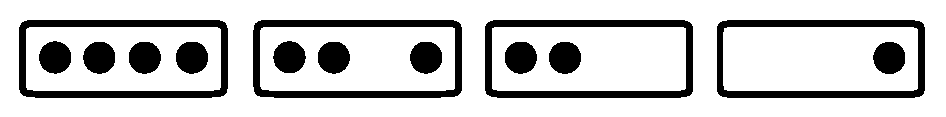
\includegraphics[width=0.4\textwidth]{img/BiometricRecordBlocks.eps}
%\caption{Pavyzdiniai biometrinių įrašų blokai. \\ Čia taškai -- įrašai, o stačiakampiai -- blokai}
%\label{img:exampleGallery}
%\end{center}
%\end{figure}

\paragraph{Darbo tikslas}

Verta pastebėti, kad UAB „Neurotechnology“ biometrinės identifikavimo sistemos darbo korektiškumas nepriklauso nuo to kuriems blokams yra priskirami biometriniai įrašai.
Tačiau darbo greitis gali kisti drastiškai.
Todėl šiam darbui keliami tikslai:
\begin{enumerate}
	\item Surasti efektyvų metodą priskirti biometrinius įrašus blokams, minimizuojant vidutinį nereikalingų biometrinių palyginimų skaičių.
	\item Surasti efektyvų metodą atrinkti blokus, kurie turi biometrinių įrašų atitinkančių biografinės užklausos predikatą.
\end{enumerate}

Nereikalingų palyginimų skaičius bus vertinamas pagal šiuos matavimus:
\begin{itemize}
	\item Dalis visų blokų, kurie turi nors vieną biografinės užklausos predikatą atitinkantį įrašą. (siekiama minimizuoti).
	\item Dalis Bloko įrašų, kuri atitinka biografinės užklausos predikatą. (siekiama maksimizuoti).
	\item Tuščias vietas esančias blokuose. (siekiama minimizuoti).
\end{itemize}

Šio darbo metu bus analizuojama kokiomis savybėmis pasižymi dažniausiai pasitaikančios biografinės užklausos.
Vėliau bus vertinama kokią įtaką darbo greičiui turi blokų užpildymas, bei blokų įrašų atitikimas vidutiniam predikatui.
Tuomet bus ieškoma metodo, padedančio optimizuoti sistemos darbą pagal ankščiau įvardintus kriterijus.



